%editors: changed title, change order of authors.

\documentclass[oribibl]{llncs}%
%TCIDATA{OutputFilter=latex2.dll}
%TCIDATA{LastRevised=Monday, November 27, 2000 11:35:04}
%TCIDATA{<META NAME="GraphicsSave" CONTENT="32">}


%\usepackage{geometry}                % See geometry.eps to learn the layout options. There are lots.
%\geometry{letterpaper}                   % ... or a4paper or a5paper or ...
\usepackage{amsmath}
%\usepackage{amsfonts}
%\usepackage{amssymb}
%\geometry{landscape}                % Activate for for rotated page geometry
    % Activate to begin paragraphs with an empty line rather than an indent. gets overruled by savestree unless savestree is modified.
\usepackage{graphicx}
%\usepackage{graphics}
%\usepackage{epstopdf}
%\usepackage{psfig}
%\usepackage[ruled]{algorithmic2e} should we try this?

%Example for automatically rescaling equations. 
% This is very tricky.
%\begin{equation}
%\label{eq:pimax}
%\resizebox{.55\textwidth}{!}{$
%\begin{split}
%P(\jtable_{2}|\set{E},\ttable) \propto &
%P(\keys = [jack,101],\it{Gr} = A, \it{Sat} = 1|\it{Int} = \class, \it{Rank} = 1, \it{Rat} = 3, \it{Diff}=1)\\
%\times & P(\keys = [jack,102],\it{Gr} = B, \it{Sat} = 2|\it{Int} = \class, \it{Rank} = 1, \it{Rat} = 2, \it{Diff}=2).
%\end{split}$
%}
%\end{equation}

%\usepackage{times}
%\usepackage[normaltitle,normalbib,normalmargins,normalindent]{savetrees}
\usepackage{amsmath}
\usepackage{amsfonts}
\usepackage{amssymb}
\usepackage{graphicx}
\usepackage{url}
%\usepackage{subfigure}
\usepackage{epstopdf}
\setcounter{MaxMatrixCols}{30}
%\usepackage{algorithm}
%\usepackage{algorithmic}
\usepackage{subfigure}
%\usepackage{subcaption}
\usepackage{fancyhdr}
\graphicspath{{../}{figures/}}
\usepackage{todonotes}

\DeclareMathOperator*{\argmax}{argmax}
\DeclareMathOperator*{\argmin}{argmin}
%\DeclareMathOperator{\pattern}{\pi}
\DeclareMathOperator{\Poly}{\mathbf{\mathrm{P}}}
\DeclareMathOperator{\RP}{\mathbf{\mathrm{RP}}}
%\DeclareMathOperator{\FP}{\mathbf{\mathrm{FP}}}
\DeclareMathOperator{\NP}{\mathbf{\mathrm{NP}}}
%\DeclareMathOperator{\E}{\mathbb{E}}
\renewcommand{\d}{\mathbf{d}}

\newcommand{\ZZ}{\mathbf{Z}}

\newcommand{\indep}{\ensuremath{\perp{}\!\!\!\!\!\!\!\perp{}}}
\newcommand{\dep}{\ensuremath{{\perp{}\!\!\!\!\!\!\!\not  \perp{}}}}
%\renewcommand{\L}{\mathcal{L}}
% variables denoting sets of nodes
\newcommand{\V}{V} 
\newcommand{\partC}{\mathcal{C}}
\newcommand{\pattern}{\pi}
% variables denoting nodes
\newcommand{\B}{B}
\renewcommand{\P}{P}
\newcommand{\R}{R}
\newcommand{\X}{X}
\newcommand{\Y}{Y}
\newcommand{\Z}{Z}
\newcommand{\F}{F}
\newcommand{\U}{U}
\newcommand{\W}{W}
\renewcommand{\S}{S}
\newcommand{\C}{C}
\newtheorem{mydef}{Proposition}
%variables for values
%\newcommand{\u}{u}
\renewcommand{\a}{a}
\renewcommand{\b}{b}
\newcommand{\z}{z}
\renewcommand{\v}{v}
\newcommand{\x}{x}
\newcommand{\y}{y}
\newcommand{\p}{p}
\newcommand{\s}{s}
\newcommand{\w}{w} % weights


%statistics
\newcommand{\divergence}{\it{D}}
\newcommand{\score}{\it{score}}
\newcommand{\confidence}{\it{conf}}
\newcommand{\support}{\it{support}}
\newcommand{\loglikelihood}{\it{LOG}}
\newcommand{\lof}{\it{LOF}}
\newcommand{\llmetric}{-L}
\newcommand{\lr}{\it{LR}}
\newcommand{\kl}{\it{KL}}
\newcommand{\el}{\it{EL}}
\newcommand{\mi}{\it{MI}}
\renewcommand{\mid}{\it{ELD}}
\newcommand{\jid}{\it{JID}}
\newcommand{\roc}{\it{ROC}}
\newcommand{\outrank}{\it{OutRank}}
\newcommand{\knn}{\it{KNNOutlier}}
\newcommand{\auc}{\it{AUC}}
\newcommand{\eld}{\it{ELD}}
\newcommand{\fd}{\it{FD}}
\newcommand{\parameter}{\theta}
\newcommand{\parameters}{\bs{\parameter}}
\newcommand{\bic}{\mathit{BIC}}
%random variables and graphical models
% number of values in the domain of a random variable
% variables for BNs
\newcommand{\domvals}{k}
\newcommand{\nodevalue}{\v}
\newcommand{\parvalue}{\mathbf{\pi}} % a single assignment of values to a set of 
%parents
\newcommand{\parvals}{l} % number of values of parent state.
\renewcommand{\r}{r} % CP-table row
\newcommand{\nbhd}{{\mathsf {nbdh}}}
\newcommand{\child}{\mathit{child}}
\newcommand{\parent}{\mathit{pa}}
\newcommand{\parents}{\mathbf{pa}}
\newcommand{\Parents}{\mathbf{PA}}
\newcommand{\family}{F} % families, family formulas
\newcommand{\vpi}{\mathbf{pa}} % for vectors of variable assignments
\renewcommand{\l}{\ell} % class label
\newcommand{\states}{r} % number of states of a variable
%\newcommand{\value}{value}
\newcommand{\mb}{\set{mb}} % markov blanket of a variable, vector-valued
\newcommand{\ssize}{N} % number of rows in join table; size of sample
\newcommand{\mbstates}{m} % number of states in Markov blanket
\newcommand{\frequency}{fr}
\newcommand{\pseudo}{\ast}
\newcommand{\counts}{+}
\newcommand{\weighted}{\ast}
\newcommand{\halpern}{H}
\newcommand{\Thetaa}{\theta}
\newcommand{\instance}{I}

%logic notation
%\newcommand{\predicate}{\phi}
\newcommand{\functor}{f}
\newcommand{\outdomain}{V}
\newcommand{\indomain}{\Omega}
\newcommand{\variable}{X} % first-order variable
\newcommand{\population}{\mathcal{P}}
\newcommand{\entity}{x}
\newcommand{\formula}{\phi}
\newcommand{\formulas}{\mathcal{\phi}}
\newcommand{\literal}{l}
\newcommand{\conjunction}{\set{C}} % conjunction of literals
\newcommand{\fterm}{\f} % open function term
\newcommand{\fterms}{F} % set of function terms, also nodes in JBN
\newcommand{\term}{\sigma}
\newcommand{\Terms}{\bs{\sigma}}
\newcommand{\constant}{a}
\newcommand{\constants}{\bs{\constant}}
\newcommand{\gterm}{g} % ground term
\newcommand{\gterms}{\bs{\gterm}} %list of ground terms
\newcommand{\vterm}{x} % variable term
\newcommand{\vterms}{\bs{\vterm}} % list of variable terms
\newcommand{\assign}{A} % assignment of values to Bayes net
\newcommand{\resultset}{\mathbb{R}}
\newcommand{\grounds}{\#}
\newcommand{\grounding}{\gamma}
\newcommand{\groundall}{\Gamma}
\newcommand{\vars}{\mathit{Var}} % variables in a conjunction
\newcommand{\igraph}{I} % instance-level dependency graph.
\newcommand{\assignment}{\set{a}}
\newcommand{\atom}{\ell}
\newcommand{\gnode}{\alpha}
\newcommand{\gfamily}{\ground{f}}
\newcommand{\numformulas}{m}
\newcommand{\structure}{\mathcal{S}}
% logic programs
\newcommand{\program}{\mathcal{B}}
\newcommand{\clause}{\mathcal{c}}
\newcommand{\head}{\mathit{head}}
\newcommand{\body}{\mathit{body}}
\newcommand{\crule}{\mathit{cr}} % combining rule
\newcommand{\level}{\mathit{level}} % rank of function symbols in LP

%datbase schema
\newcommand{\rcolumns}{R}
\newcommand{\ecolumns}{E}
\newcommand{\dtable}{T} % can't use \table. Generic database table
\newcommand{\datatable}{D} % generic data table, not necessarily part of database.
\newcommand{\jtable}{J} % join table
\newcommand{\Ejoin}{$J^{+}$}
\newcommand{\jtables}{m}
\newcommand{\rtable}{R} % relationship table
\newcommand{\etable}{E} % entity table.
\newcommand{\ttable}{X} % target table
\newcommand{\nextended}{n}
\newcommand{\row}{r}
\newcommand{\rows}{\mathit{rows}}
\newcommand{\col}{j}
\newcommand{\cols}{\mathit{cols}}
\newcommand{\unary}{\f} % to denote a unary or attribute function
\newcommand{\numatts}{u} % to denote the number of unary or attribute functions.
\newcommand{\g}{g} % alternative for function
\newcommand{\relational}{\mathbf{r}} % denotes a generic relational functors, can be both relationship or descriptive attribute of relationship
\newcommand{\Relation}{R} % denotes a generic boolean relation
% a special type of literal conjunction that assigns a value %to each variable
\providecommand{\keywords}{\textbf{keywords: }}
\newcommand{\loss}{\ell}
\newcommand{\class}{c} % the class attribute
\newcommand{\classlabel}{y} % the class label
\newcommand{\classifier}{\mathcal{M}}
\newcommand{\target}{t} % target object
\newcommand{\Target}{T}
\newcommand*\rfrac[2]{{}^{#1}\!/_{#2}}
\newcommand{\object}{o}
\newcommand{\Class}{C}
\newcommand{\scorediff}{\Delta}
\newcommand{\model}{B}
\newcommand{\modelprob}{\theta}
\newcommand{\profile}{P}
% the probabilities defined by a model, like conditional probabilities in a BN
\newcommand{\Targetcount}{\Gamma}
\newcommand{\neighbor}{n}
\newcommand{\feature}{V} % feature or desc attribute of object or link
\newcommand{\features}{\bs{v}} % features 
\newcommand{\Features}{\bs{V}}
\newcommand{\attribute}{a} % nonclass attribute of target object
\newcommand{\attributes}{\bs{a}}
\newcommand{\rels}{\bs{R}} % chain of relationships.
\newcommand{\maxpath}{\rho}
\newcommand{\eatts}{\it{1Nodes}}
\newcommand{\ratts}{\it{2Nodes}}
\newcommand{\atts}{\it{ANodes}}
\newcommand{\marginalize}{\it{margin}}
%special functions
\newcommand{\AVG}{\it{AVG}}
\newcommand{\instances}{n} % counts number of occurrences in DB
\newcommand{\prob}{p} % frequency of formula true in in DB

%variables denoting graphs or models
\newcommand{\mln}{M}
\newcommand{\G}{G}
\newcommand{\node}{V}
\newcommand{\nodes}{V}
\newcommand{\edges}{E}
\newcommand{\clique}{C}
\newcommand{\cliques}{\mathcal{\clique}}
\newcommand{\cliquevalue}{c}
\newcommand{\graph}{G}
\newcommand{\M}{M}
\newcommand{\J}{J}
\renewcommand{\H}{H}
\newcommand{\K}{K} % component
\renewcommand{\O}{O} % oracle
\renewcommand{\path}{\rho} % path, also foreignkey path
% Markov nets
\newcommand{\potential}{\Psi}
% database schema
\newcommand{\type}{\tau} % to denote a generic type
\newcommand{\E}{E} % for entity tables
\newcommand{\e}{e} % for specific entities
\newcommand{\f}{f}
\newcommand{\new}{\it{new}}
\renewcommand{\c}{c}
\renewcommand{\R}{R} % for relationship tables
\newcommand{\A}{A} % for attributes
\newcommand{\T}{T} % for tables generically
\newcommand{\New}{N}
\newcommand{\D}{\mathcal{D}} % for database instance
\newcommand{\databases}{\set{D}} % the number of databases
\newcommand{\vocab}{\mathcal{\L}} % for logical vocabulary associated with database
\newcommand{\name}{\mathit{name}} % generic attribute
\newcommand{\dom}{\mathit{dom}} % domain of attributes
\newcommand{\etables}{\alpha} % entity tables
\newcommand{\rtables}{\beta} % relationship table number
% specific constructs for examples


\newcommand{\team}{\it{T}}
\newcommand{\player}{\it{P}}
\newcommand{\match}{\it{M}}


\newcommand{\director}{\it{Director}}
\newcommand{\movie}{\it{Movie}}
\newcommand{\user}{\it{User}}
\newcommand{\corr}{\it{\rho}}
\newcommand{\student}{\mathit{Student}}
\newcommand{\I}{\mathit{I}}
\newcommand{\course}{\mathit{Course}}
\newcommand{\prof}{\mathit{Professor}}
\newcommand{\person}{\mathit{Person}}
\newcommand{\TA}{\mathit{TA}}
\newcommand{\actor}{\mathit{Actor}}
\newcommand{\age}{\mathit{age}}
\newcommand{\intelligence}{\mathit{intelligence}}
\newcommand{\diff}{\mathit{difficulty}}
\newcommand{\reg}{\mathit{Registered}}
\newcommand{\win}{\it{win}}
\newcommand{\ra}{\mathit{RA}}
\newcommand{\bt}{\mathit{blood type}}
\newcommand{\grade}{\mathit{grade}}
\newcommand{\gpa}{\mathit{gpa}}
\newcommand{\jack}{\mathit{Jack}}
\newcommand{\jill}{\mathit{Jill}}
\newcommand{\smith}{\mathit{Smith}}
\newcommand{\cmpt}{\mathit{CMPT120}}
\newcommand{\hi}{\mathit{Hi}}
% various constants
\newcommand{\true}{\mathit{T}}
\newcommand{\false}{\mathit{F}}
\newcommand{\normalconstant}{Z} % the normalization constant

% orderings
\newcommand{\pred}{\mathit{pred}}
%procedure names and such
\newcommand{\join}{\textsc{Join-Frequencies}}
\newcommand{\linus}{\textsc{Linus }}
\newcommand{\foil}{\textsc{Foil }}
\newcommand{\MLN}{\textsc{MLN}}
\newcommand{\treetilde}{\textsc{TILDE }}

%%%
%undirected models
\newcommand{\pot}{\phi} % potential function
%\newcommand{\theHalgorithm}{\arabic{algorithm}}
\newcommand{\test}{test}
\def\set#1{\mathbf{#1}}
\def\bs#1{\boldsymbol{#1}}
\def\ground#1{\overline{#1}}


\DeclareGraphicsRule{.tif}{png}{.png}{`convert #1 `dirname #1`/`basename #1 .tif`.png}
%\usepackage{icml2008}
%\usepackage{mlapa}
\usepackage{url}
%\usepackage{caption}
%\usepackage{subfigure}
%\usepackage[normaltitle,normalmargins]{savetrees}
% don't mess with the bibliography
%\usepackage{setspace}
% for bibliography spacing. doesn't work for some reason
% the following shrinks space in bibliography, instead of the spacing command.
\let\oldthebibliography=\thebibliography
  \let\endoldthebibliography=\endthebibliography
  \renewenvironment{thebibliography}[1]{%
    \begin{oldthebibliography}{#1}%
      \setlength{\parskip}{0ex}%
      \setlength{\itemsep}{0.1ex}%
  }%
  {%
    \end{oldthebibliography}%
  }
% nodes


\newcommand{\team}{T}
\newcommand{\player}{P}
\newcommand{\match}{M}
\newcommand{\plusminus}{\mbox{+/-}}
%\newcommand{\true}{\mathrm{T}}
%\newcommand{\false}{\mathrm{F}}

%\newcommand{\functor}{f}
\newcommand{\aggregate}{\it{agg}}

\newtheorem{observation}{Observation}

%\def\sitem{\vspace{-1.2em} \item} % to shrink space between items
\def\seq#1{\langle#1\rangle} % only in math
\def\here#1{{\bf $\langle\langle$HERE:\ #1$\rangle\rangle$}}
\def\ie{{\em i.e.},\ }
\def\eg{{\em e.g.},\ }
\def\set#1{\mathbf{#1}}
%% try to get rid of paragraphs ending in single words
%\looseness = -1

%%reduce space between paragraphs
%\addtolength{\parskip}{-1.5mm}

%%reduce space around floats. Problem seems to be the first figure
%\addtolength{\intextsep}{-1mm}

%\vskip 0.3in



\institute{School of Computing Science,   Simon Fraser University,\\ Burnaby,
B.C.,   Canada~V5A~1S6,   \email{oschulte@cs.sfu.ca,kdr4@sfu.ca}   }
\newtheorem{axiom}[theorem]{Axiom}

\begin{document}

\title{Aggregating Predictions vs. Aggregating Features for Relational Classification: A Comparison}
\author{Oliver Schulte
\and Kurt Routley}
\maketitle


\begin{abstract} This paper presents a fast, principled, and accurate method for leveraging standard machine learning classifiers for relational classification. The method uses the average of a classifier score over a target's relational neighbourhood as an aggregate classifier score. We show that the average is consistent with the classic random selection semantics for probabilistic logic. Our experiments compared different relational classifiers on sports data. Compared to propositionalization methods and other score aggregators, the random selection classifier showed robust and competitive performance. 
\end{abstract}


\section{Introduction} Most real-world structured data are stored in the relational format, with different types of entities and information about their attributes and links between the entities.
Relational data classification is the problem of predicting a {\em class label} of a target entity given information about features (attributes) of the entity, of the related entities, or neighbors, and of the links. This paper presents a fast, principled, and accurate method for leveraging standard machine learning classifiers for relational classification.

A key challenge for relational classification is that the number of links of the target entity is not uniformly bounded. Since the features of each neighbor potentially carry information about the target class label, the number of predictive features for classification is thus a function of the size of the target entities neighborhood, rather than a fixed dimensionality $d$. Relational classifiers therefore aggregate the information from the target entity's neighborhood. There are two fundamental options for aggregation: 1) First aggregate the neighbors' features into a single aggregate feature vector, then classify based on the aggregate vector. 2) First derive a classification score based on a single neighbor, then aggregate the scores. 
%Figure~\ref{fig:classify} illustrates these options schematically.
%
In this paper we compare the two approaches empirically on data sets with continuous features. Since standard relational benchmark datasets contain discrete features mainly or only, we use two real-world continuous datasets that summarize players' actions in ice hockey and in soccer. The ice hockey dataset was obtained by a web crawler and has not been analyzed before.

%\begin{figure}[htbp]
%\begin{center}
%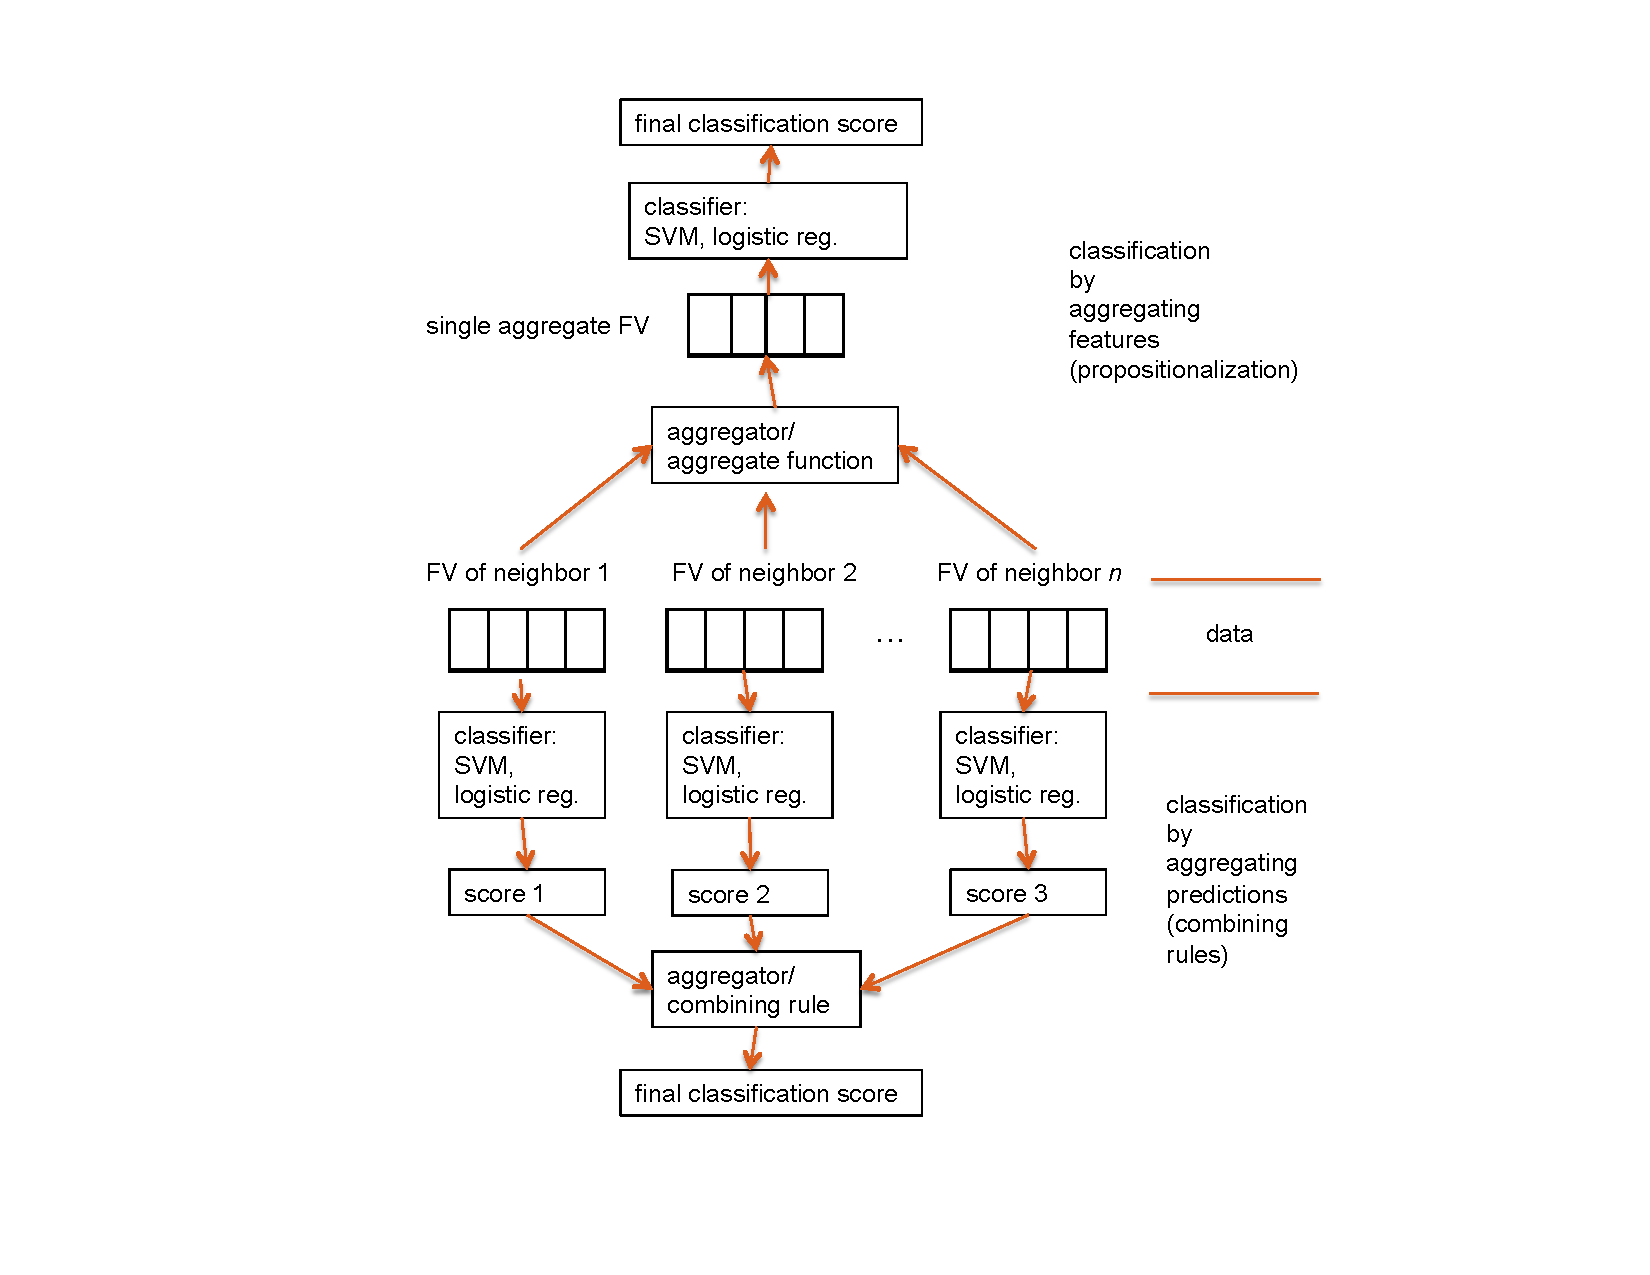
\includegraphics[width = 1 \textwidth]{figures/classify}
%\caption{Two different approaches to relational classification. FV = feature vector. The problem is to predict a class label for a target entity. The data provide a feature vector for each entity related to the target entity (neighbors $1,\ldots,n$). (We omit features of the target entity for simplicity.) Top: aggregating features combines the $n$ feature vectors into a single one, then applies a standard nonrelational classifier to predict a class label. Bottom: aggregating predictions applies a standard nonrelational classifier to each feature vector to obtain $n$ classification scores (e.g. positive class probabilities). A combining rule aggregates the $n$ scores to predict a class label.}
%\label{fig:classify}
%\end{center}
%\end{figure}

%In addition to evaluating standard methods for aggregating features and predictions, we 
%We propose a new log-linear method for aggregating predicted class probabilities, using the mean of the log-class probabilities geometric mean. This aggregation method is equivalent to computing the expected log-class probability given a {\em randomly chosen} neighbour of the target entity. Random selection classification is consistent  with the classic random selection semantics of probabilistic 1st-order logic due to Halpern and Bacchus \cite{Halpern90,Bacchus90}. 
%Within a loss-minimization framework, training a classifier for random selection classification can be done by minimizing the expected classifier loss, defined as the expected loss from randomly selecting a neighbour predicting the class label based on the selected neighbour. 
Computionally, classifier training with score aggregation can be done very simply by forming a data table such that one row contains the features of one neighbor, and applying a regular non-relational learning algorithm to this table.\footnote{If the neighbourhood sizes of different target entities differ, a simple adjustment of the classifier loss for neighborhood size is necessary, see details below.} 
%We show that training a classifier on such a data table minimizes the expected random selection classifier loss.


\paragraph{Evaluation.}
We use standard aggregation functions to aggregate continuous features (mean, sum, min, max). Once features have been aggregated, any standard single-table machine learning classifier for continuous features can be applied for classification. In this paper we apply logistic regression and support vector machines (SVMs). 

Both logistic regression and SVMs return a continuous classification score. We apply the single-table classifier to the features of each neighbor to obtain a classification score for the neighbor, then aggregate the scores. For aggregating scores, we use the same functions as for aggregating features.  In addition we apply noisy-or, a standard rule for combining a list of probabilities into a single probability.
%, and our new method, the mean of log-probabilities (equivalent to the geometric mean\footnote{The geometric mean of $x_{1},\ldots,x_{n}$ is $(\prod_{i} x_{i})^{1/n}$.}).

The basic task is to predict the result of a given target team in a given target match (win or not). We examine hockey data from the NHL and soccer data from the UK Premier League. The training set contains data from previous matches and the test set data from the following ones. We experiment with two different feature sets: First, summary statistics from the previous season for each player (e.g., number of goals scored by the player). Second, in addition, the action counts for each player on the target team in the target match. 

Our main conclusion is that among score aggregation operators, the average or mean provides robust competitive performance across different settings. We show that the average operator is consistent  with the classic random selection semantics of probabilistic 1st-order logic due to Halpern and Bacchus \cite{Halpern90,Bacchus90}. The performances of the best score and feature aggregation methods is close except for one dataset where feature aggregation is clearly superior. We outline a hybrid approach that combines informative aggregate features with score-based classification.


\paragraph{Contributions.}

Our main contributions may be summarized as follows.

\begin{enumerate}
\item The first direct comparison of feature aggregation vs. score aggregation methods for relational classification.
\item A new score aggregation method that uses the expected classification score from a random selection of the target node's neighbour. 
%Training a classifier for this classification score can be done using the same techniques as for nonrelational classification.
\item A new real-world dataset in relational database format with play summaries from 3,857 NHL matches, available on-line from \url{ftp://ftp.fas.sfu.ca/pub/cs/oschulte/hockey}.
\end{enumerate}


\section{Related Work} Because of the importance of relational data, there has been much work on link-based classification. For overviews please see \cite{han2009,Bina2012}. We provide a high-level description of the work most relevant to the question of feature vs. score aggregation.

\paragraph{Aggregating Classifier Scores.} Most approaches that aggregate classification scores use a function that maps a list of probabilities to a single probability. Following the terminology of Bayes nets, such functions are referred to as {\em combining rules} \cite{Pearl1988,Kersting2007}. In our terminology, a combining rule is a special kind of classifier score aggregation. 
%We use the more general concept, because some of our experiments aggregate scores that are not probabilities (e.g., the outputs of SVMs), and some aggregate probabilities but map them to a number that is not itself a probability (e.g, the geometric mean is not normalized). 
While the arithmetic mean of class probabilities has been considered for aggregating probabilities in relational learning \cite{Natarajan2008}, the geometric mean is a new proposal motivated by the random selection semantics. The random selection semantics is a classic concept from AI research that combines 1st-order logic with probabilities \cite{Halpern90,Bacchus90}. The key idea is to interpret a free 1st-order variable as a random variable that randomly selects an element from its domain. The random selection semantics was previously applied for learning generative Bayes net models \cite{Schulte2011}. To our knowledge we present the first application to relational discriminative learning.\footnote{A related previous paper was presented at the 2012 UAI-StarAI workshop.
 %\cite{Schulte2012d}. 
 The nonarchival workshop did not publish proceedings. 
%This paper used the random selection semantics to define a Gibbs conditional probability of a target node conditional on its Markov blanket. Differences with the current paper include: (i) Only discrete features were considered, and no feature aggregation. (ii) Only Bayes net models were considered. (iii) The learning problem was parameter learning for Bayes nets, not general relational classification.
}

\paragraph{Propositionalization.} The majority of work on relational classification has adopted the feature aggregation strategy. 
%strategy of aggregating the features of a target entity's neighbor into a single feature vector of the target entity. 
This approach of ``flattening'' the relational structure is generally known as {\em propositionalization} \cite{Kramer2000}. %To our knowledge, ours is the first comparison of the approach of using classifier score aggregation or combining rules vs. propositionalization.
%
For continuous features, propositionalization methods use the same standard aggregate functions that we use in this paper \cite{Krogel2002,C.Vens2004}. For discrete data, a common approach is to use a {\em feature function}. A feature function maps a relational neighbourhood to a single value for the given feature. For instance, if the feature is ``student's grade is A'', the count feature function returns the number of A's achieved by the student. If the feature function returns a continuous or integer value, the values of the feature functions are used as inputs to a log-linear model (conditional random field) for prediction \cite{Sutton2007,Taskar2002,Domingos2009,Lu2003}. A feature function may also return a discrete value; a commonly used binary feature function is existential quantification, for example using 1 as a classifier if the student has achieved an A in some course, and a 0 otherwise.

\paragraph{Complex Features.} The most expressive propositionalization models apply feature functions to combinations of the discrete features given in the data (e.g., \cite{Kuzelka2011}). For instance, to predict the ranking of a student, we may distinguish the number of A grades achieved in higher-level course from those achieved in lower-level courses. Complex discrete features may be combined with aggregation functions, as aggregation conditions, for continuous variables  \cite{C.Vens2004,Popescul2007}. For example, to predict the age of a user in a social network, we may consider the average age of her friends who have the same gender and live in the same city.

Several researchers discuss advantages and disadvantages of  propositionalization for link-based classification \cite{DavidJensen2002,han2009}. 
%Propositionalization has the advantages and disadvantages of general predicate invention approaches. 
The main advantage is expressiveness: feature generation methods search a large space of potentially useful features. If an informative new complex feature or aggregate feature can be found, it improves classification performance and informs the user. The disadvantages are problems with both statistical and computational efficiency. Aggregation loses information in the data, which increases the variance of classifier estimates and causes problems with both type 1 and type 2 errors in feature selection \cite{Jensen2002a}. Searching a large space of potential features presents considerable computational challenges. For an example, generating 100,000 features on the standard CiteSeer dataset, can take several CPU days
\cite[Ch.16.1.2]{Popescul2007}). Compared to feature generation, the score aggregation approaches we describe in this paper provide a simple and fast baseline for link-based classification. At the end of the paper we describe possibilities for combining score-based aggregation with feature generation.

\paragraph{Sports Statistics.} The problem of predicting the results of sports matches has received considerable attention for different sports. For an overview please see \cite{Schumaker2010}. We do not claim that the methods in this paper are competitive for predicting the match results. 
%For instance, the goal is usually to predict the result of a match before the game is played, so  the action counts of players in the target game are not available. 
We use the NHL data as a real-world dataset in an interesting domain with interpretable features for comparing aggregating features vs. aggregating predictions.

\section{Notation and Data Format} We introduce notation to discuss relational features and data and to support theoretical analysis. We follow the functor-based notation for combining statistical and relational concepts due to Poole \cite{Poole2003}.

\paragraph{Functor Features.}
A \textbf{population} is a set of individuals, corresponding to a domain or type in logic. A \textbf{feature} is of the form $f(t_{1},\ldots,t_{k})$ where $f$ is a functor (either a function symbol or a predicate symbol) and each $t_{i}$ is a first-order variable or a constant. Each feature has a set of values (constants) called the \textbf{domain} of the feature. 
A feature whose range are the truth values $\{\true,\false\}$ is a \textbf{predicate}. 
Predicates are usually written with uppercase Roman letters, other feature with lowercase letters.
A \textbf{grounding} replaces each 1st-order variable in the feature by a constant; the result is a ground feature. A grounding may be applied simultaneously to a set of features. One of the features is the class or \textbf{target} feature. A grounding of the target feature is a \textbf{target instance}.

\paragraph{Examples.} In our datasets the basic populations are teams, players, matches, with corresponding first-order variables $\team, \player, \match$. Examples of features include the following.

\begin{itemize}
\item $\it{result}(\team,\match)$ denotes the result of a team in a match (win or lose). This is the target feature.
\item The ground feature $\it{result}(Canucks,1)$ denotes the result of the Canucks in match 1. This is a target instance.
\item $\it{PlaysFor}(\player,\team,\match)$ is a predicate that is true if player $\player$ plays for team $\team$ in match $\match$.
\item $\it{goals}(\team,\player,\match)$ is the number of goals scored by a player of a given team in a match.
\item $\plusminus(\player,\match)$ is the $\plusminus$ score of a player in a match. This is a  common measure of the player's performance; for precise definition see $\cite{Schumaker2010}$.
\end{itemize}

\paragraph{Aggregation.} Given a feature $\functor$, an aggregate function $\aggregate$ applies to one of the argument variables of $\functor$. We use the subscript notation $\aggregate_{X}$ to indicate that variable $X$ is the object of aggregation \cite{Popescul2007}. The result is a feature with one less argument. Examples include the following.

\begin{itemize}
\item $\it{goals}(\team,\match) \equiv \sum_{\player} \it{goals}(\team, \player,\match)$ is the number of goals scored by a team in a match.
\item $\it{past}\_\it{goals}(\player) \equiv \sum_{\match \mbox{ in past season}} \it{goals}(\team, \player,\match))$ denotes the sum of a player's goals in the past season.
%\item $\it{Past}\plusminus(\player) \equiv \sum_{\match \mbox{ in past season}} \plusminus(\player,\match)$ denotes the sum of a player's $\plusminus$ scores in the past season.
\end{itemize}

%The aggregation functions that we use in this paper are max, min, sum, midpoint, average (arithmetic mean), geometric mean. 

%Suppose that we fix a \textbf{target feature} for prediction, e.g. $\it{result}(\team,\match)$. A set of features is propositionalized if only the 1st-order variables in the target feature appearing in the features in the set. For instance, $\it{goals}(\team,\match)$ is propositionalized, whereas $\it{Past}\plusminus(\player)$ is not.
%
%The simple Bayes net of Figure~\ref{fig:bn} illustrates link-based classification using the functor notation. (Bayes net with child = result, parents = plusminus(player), goals(team,match), goals(team,match,player), plays for). The random selection semantics for Bayes nets with functors views each 1st-order variable as a \cite{Schulte2013} random selection from its domain. Since a function of a random variable is also a random variable, this means that the functors in the Bayes net are also random variables. For instance, suppose that the Bayes net parameters specify the conditional probability [come up with example]. In the random selection semantics, this probability statement can be interpreted as ``[spell out]''.

\paragraph{Relational Data Tables.}
Relational data can be visualized in terms of the \textbf{groundings data table}. The data table has one column for each feature. It has one row for each simultaneous grounding of all functor features where the instances of the nonclass features are in the neighborhood of the instance of the target feature. Thus if the target functor feature is instantiated with ground instance $\target$, the data table contains a row listing the attributes of each neighbor $\neighbor$ of $\target$. Tables~\ref{small-join} and~\ref{small-aggregate} (propositionalized) show an example of  groundings data tables. As the examples illustrate, aggregation increases the number of features (columns) and decreases the number of data points (rows). 

%\marginpar{add column for score to data table}

\begin{table}[htbp]
\caption{Data Table for NHL. Features include last season aggregates  and target match statistics for players.}
\begin{center}
\begin{tabular}{|l|r|l|l|r|r|}
\hline
result(\team,\match) & \multicolumn{1}{l|}{MatchId \match} & TeamId \team & PlayerId \player& \multicolumn{1}{l|}{past\_goals(\player)} & \multicolumn{1}{l|}{goals(\team,\player,\match)}\\ \hline
Loss & 2010020023 & Canucks & D. Hamhuis & 5 & 0\\ \hline
Loss & 2010020023 & Canucks & D. Sedin & 34 & 0\\ \hline
Loss & 2010020023 & Canucks & H.Sedin & 32 & 0\\ \hline
... & %\multicolumn{1}{l|}{} 
...& ...  & (Player \#18) & ... & ... %\multicolumn{1}{l|}{}  \multicolumn{1}{l|}{} \\ \hline
\\\hline
Win & 2010020033 & Canucks & D. Hamhuis & 5 & 0\\ \hline
Win & 2010020033 & Canucks & C. Ehrhoff & 17 & 0\\ \hline
Win & 2010020033 & Canucks & H. Sedin & 32 & 0\\ \hline
\end{tabular}
\end{center}
\label{small-join}
\end{table}

\begin{table}[htbp]
\caption{Data Table for NHL. Features are team aggregates of last season player aggregates and aggregates of player target match statistics.}
\begin{center}
\begin{tabular}{|l|r|l|r|r|}
\hline
result(\team,\match) & \multicolumn{1}{l|}{MatchId \match}  & TeamId \team & \multicolumn{1}{l|}{Sum\_past\_goals(\team)} & \multicolumn{1}{l|}{Sum\_goals(\team,\match)} \\ \hline
Loss & 2010020023 & Canucks & 252 & 1\\ \hline
Win & 2010020033 & Canucks & 259 & 2\\ \hline
\end{tabular}
\end{center}
\label{small-aggregate}
\end{table}


\section{Score Aggregation and Random Selection Classification} For simplicity, we discuss score aggregation for a single relationship, which defines a neighborhood for each grounding of the target feature. Our discussion applies equally to classification scores obtained with different types of neighbourhoods. Score aggregation can be visualized in terms of the \textbf{groundings data table}, or data table for short. 

Suppose that we have trained a classifier model $\classifier$ that returns a classification score for a given target label $\classlabel$ and feature vector $\features$. We write $\score_{\classifier}(\classlabel;\features)$. We can apply this classifier to each row in the groundings data table to derive a classification score from the features of each neighbour of a given target instance $\target$.
%
Given a list of classification scores, one for each row in which the target instance appears in the data table, we can apply a standard aggregation function to obtain an overall classification score. We also use the noisy-or rule for combining probabilities \cite{Kersting2007}.

%When the classification scores represent probabilities, a common way to combine them is to use the ``noisy-or'' rule: [give definition]
%
%Intuitively noisy-or is a soft version of the disjunctive truth function: if any one of the probabilities is above 0.5, the combined probability is likely to be above 0.5.

\paragraph{Random Selection Semantics} We can also apply the classic random selection semantics to derive a score aggregation method in a principled way \cite{Halpern90,Bacchus90}. Consider a probabilistic classifier score such as 

$$0.7 = P_{\classifier}(\it{result}(\team,\match) = loss; \it{past\_goals}(\player) = 10, \it{goals}(\team, \player,\match)= 2)$$

On the random selection semantics, the meaning of this statement is ``if we were to randomly select a team, match, and player, there is a 0.7 probability that the class label is loss.'' With this interpretation, for a fixed target instance $\Target = \target$, the \textbf{random selection classification score}  is the expected or {\em average} score over all the neighbours of the target instance. In terms of the data table, it is the average of the scores in the rows in which the target instance appears. Therefore {\em the random selection semantics leads to using the arithmetic mean for score aggregation.} 

We can also use the random selection semantics for learning, not only prediction.  A common framework for learning a classifier is to tune the classifier's parameters to minimize a loss function.  For example, for probabilisic classifiers, a common loss function for a single data vector with class label $\classlabel$ and features $\features$ is the log-likelihood loss $\loss_{\classifier}(\classlabel;\features) = -\ln P_{\classifier}(\classlabel;\features)$. In terms of the data table, for a given classifier there is a loss in each row just as there is a score. Therefore the classifier's \textbf{random selection loss} on a single target instance is the average loss over the target's neighbours. The random selection loss on the entire dataset is the sum of the losses for each single target instance. 

In comparison, given a data matrix as input, an optimization algorithm would assess the loss for each row, then sum the losses for each row.  Without adjusting for neighbourhood sizes the summation loss is biased towards target instances with larger relational neighbourhoods. These observations have statistical and computational significance.  

(1) One of the difficulties with applying standard loss minimization to relational data is that relational datapoints are not i.i.d., but the standard summation of classifier loss over data points assume  data point independence. The random selection concept can be applied to define, in a principled way, a loss for an entire relational data table, based on a loss function for a single row.  

(2) Adjusting the loss function for the size of different neighbourhoods requires only a small adjustment in the design of a standard classifier algorithm. If all target instances have the same number of neighbours, it is not necessary, and we can apply a standard classifier algorithm to the groundings data table.

Next we present empirical evaluation of feature and score aggregation methods.

%
%\subsection{Random Selection Classification}
%The random selection semantics suggests using the arithmetic mean for score aggregation for the following reason. On the random selection semantics, the classification scores of the classifier $\classifier$ can be interpreted as follows: For a randomly selected object $\Target$ and a randomly selected feature vector $\Features$, the classification score for $\class(\Target) = \classlabel$ given that $\Features =  \features$ is given by $\score_{\classifier}(\classlabel;\features)$. Therefore for a fixed target instance $\Target = \target$, the \textbf{random selection classification score}  neighbor is given by the expectation
%
%\begin{equation} \label{eq:exp-score}
%E[\score_{\classifier}(\classlabel)] \equiv \frac{1}{|\nbhd(\target)|} \sum_{j=1}^{|\nbhd(\target)|} \score_{\classifier}(\classlabel;\features_{j}) 
%\end{equation}
%where $\nbhd(\target)$ is the set of neighbours of the target instance, and $\features_{1},\ldots,\features_{|\nbhd(\target)|}$ is a list of the neighbours' features. The expression on the right hand side is the mean of the classification scores.
%
%
%\subsection{Random Selection Loss Function} A common framework for learning a classifier is to tune the classifier's parameters to minimize a loss function. One of the difficulties with applying standard loss minimization to relational data is that relational datapoints are not i.i.d., but the usual definitions of classifier loss on a dataset assume  data point independence. For example, for probabilisic classifiers, a common loss function for a single data vector with class label $\classlabel$ and features $\features$ is the log-likelihood loss $\loss_{\classifier}(\classlabel;\features) = -\ln P_{\classifier}(\classlabel;\features)$ where $P_{\classifier}(\classlabel;\features)$ denotes the probability that the classifier assigns to $\classlabel$ given as input $\features$. Given independent data rows, the class probabilities for different rows are independent of each other, and therefore the single instance loss function can be extended to the entire data table by summing the classifier losses for each row. However, relational data are not i.i.d. For example in the groundings data table, the labels of the match are the same in different rows for the same match. More generally, there are dependencies between the attributes of different entities \marginpar{cite something} 
% The random selection concept can be applied to define, in a principled way, a loss for an entire relational data table, based on a loss function for a single row.  The basic idea is to use the expected loss of a classifier given a random selection of a target instance and of a neighbour. This  expected value is well-defined even for dependent data.  Formally, we define the \textbf{random selection loss} on a dataset as follows. Let $\loss_{\classifier}(\classlabel;\features)$ denote the loss of the classifier when a prediction is derived from the input features $\features$ and the true class label is $\classlabel$. 
%% Given the random selection semantics, we can define the  of a classifier as the expected loss given a random selection of a target instance and of a neighbor. The formal definition is as follows.
%
%\begin{equation} \label{eq:exp-score}
%E[\loss_{\classifier}(\D)] \equiv \frac{1}{\Targetcount} \sum_{\target=1}^{\Targetcount} \frac{1}{|\nbhd(\target)|} \sum_{j=1}^{|\nbhd(\target)|}\loss_{\classifier}(\classlabel_{\target};\features_{j}) 
%\end{equation}
%
%where $\Targetcount$ is the number of ground instances of the target feature. In comparison, given a data matrix as input, an optimization algorithm would assess the loss for each row, then sum the losses over the rows. So given the groundings data table as input, the classification algorithm would compute the loss as
%
%\begin{equation} \label{eq:classifier-loss}
%\sum_{\target=1}^{\Targetcount} \sum_{j=1}^{|\nbhd(\target)|}\loss_{\classifier}(\classlabel_{\target};\features_{j}) 
%\end{equation}
%
%Comparing equations~\eqref{eq:classifier-loss} and~\eqref{eq:exp-score}, the constant $\frac{1}{\Targetcount}$ does not change the loss minima, and therefore the only relevant difference between the random selection loss and the standard summation loss is that the random selection loss scales the contribution of each target instance by the size of its neighborhood. Without such scaling the summation loss is biased towards target instances with larger relational neighbourhoods. We draw the following conclusions from this analysis of the random selection semantics for classification.
%
%\begin{enumerate}
%\item  The random selection classification score for a target instance is the mean of the classification scores derived from the neighbours of the target instance.
%\item If all target instances have the same number of neighbours, we can apply a standard classifier algorithm to the groundings data table. The reason is that the standard summation loss that a classification algorithm would compute from the groundings data table is equivalent to the random selection classifier loss.
%\item If  target instances differ in the number of neighbours, the random selection loss is equivalent to averaging the losses for each target instance. This requires only a small adjustment in the design of a standard classifier algorithm.
%\end{enumerate}
 
% In our experiments below, the relational neighbourhoods all have the same size, since the number of players per team per match is constant. Therefore the random selection semantics provides a theoretical justification for applying standard classification algorithms directly, even though there are dependencies between different rows of the data table.



\section{Evaluation} Each method is evaluated by its ability to correctly classify the result based on the features supplied. For feature aggregation, this involves aggregating the supplied features and using these aggregated features to train a SVM or Logistic Ridge Regression model and return a result (win or loss) classification for each team per match. 
%The maximum classification accuracy of each feature aggregation model is recorded in Table~\ref{table:feture-aggregation-results}.

For score aggregation, all features are first used to train a SVM or Logistic Ridge Regression model to learn a score for each row of features for a player in a given match. These player scores are then grouped for each team in a match, and the scores are aggregated to generate a team score and result classification.

%The precision, negative prediction value, sensitivity, and specificity are also recorded to evaluate each model.
%
%\subsection{Hypotheses} A nice way to structure this section and to engage the referees is to give a list of what you want to establish through your experiments, before you give the details of your experiments. This usually also clarifies things for yourself. Hopefully you have more interesting hypotheses to test than ``I can find some datasets on which the predictive accuracy of my system is higher than that of some previous methods.'' The following conjecture will be evaluated:
%\begin{enumerate}
%\item Score aggregation will perform better than feature aggregation. The intuition is that aggregating features loses the information from individual player performance. By first evaluating players individually and then aggregating player scores, an improved measure of team scores can be obtained.
%\end{enumerate}
%SELF NOTE: May need to add more conjectures to this section.
%
\subsection{Hardware and Software} The learning algorithms were executed with 64-bit Windows 7 with 12GB RAM and an Intel Core i7 2670QM CPU 2.2GHz processor. For Logistic Ridge Regression we used the L1General Matlab code \cite{bib:l1general}. For Support Vector Machine training we used the LibSVM software version 3.17.
%\cite{libsvm}.

%Logistic Ridge Regression tests were completed using Java and Weka on CentOs 6.4 with 4GB RAM and an Intel Core 2 Duo CPU E6550 2.33GHz processor. Logistic Ridge Regression and SVM tests were also performed using Matlab and code from Mark Schmidt on 64-bit Windows 7 with 12GB RAM and an Intel Core i7 2670QM CPU 2.2GHz processor.

\subsection{Datasets}

We prepared data tables from NHL and Premier League data. The target feature is $\it{result(Team,Match)}$. A positive classification means that the team is predicted to lose the match. In the NHL, no ties are possible. In the Premier League dataset, we removed 90 tied matches from 380 total matches to obtain a comparable binary classification problem.

\subsubsection{NHL data tables}

We used the webcrawler Selenium \cite{bib:crawler} to download player game statistics (Box Scores) from \url{http://www.nhl.com/gamecenter/} for the seasons 2009--2013. The box scores summarize player statistics for each match, a total of 13 continuous-valued features. We only consider skaters, no goalies. We refer to these as \textbf{match statistics}. The match features include goals, assists, plus-minus, penalty minutes, and total time on ice. For each player, we sum his match statistics over all NHL games in the previous season, to obtain a total of 13 season totals. In addition, we add 5 other season statistics: number of games played, game winning goals, powerplay goals, shorthanded goals, and shot percentage. We refer to the resulting 18 features as \textbf{last-season statistics}. From this data we prepared the following 4 data tables, one for each choice of (aggregate/not aggregate) and (last-season/all features).

\begin{description}
\item[Last Season] A row in this table corresponds to a match, one of the teams involved in the match, and one player who played for that team in the match. Each NHL team dresses exactly 18 skaters per match, so for a given match, the data table contains $2 \times 18 = 36$ rows. The 19 columns represent the result of the match, and the 18 last-season statistics of the player.
\item[All Features] This data table contains the last season features and the match statistics.
%So for each match, we have 36 rows as in the Last Season dataset, and we have $19+13 = 37$ columns.
Table~\ref{small-join} illustrates this design.
\item[Last Season Aggregate] We apply the 6 aggregate functions max, min, sum, midpoint, average (arithmetic mean), geometric mean to each last-season feature.
%The data table contains two rows for each match (one per team), and $1+6 \times 18 = 109$ columns.
\item[All Features Aggregate] Same as All Features Aggregate but with aggregates of match statistics as well.
%The total number of columns is therefore $1+108+6 \times 13 = 187$ columns.
Table~\ref{small-aggregate} illustrates this design.
\end{description}

%\begin{table}[htbp]
%\caption{Training data for NHL Last Season and Target Match Features with Match Result}
%\begin{tabular}{|l|r|l|l|r|r|r|r|}
%\hline
%Result & \multicolumn{1}{l|}{MatchId} & TeamId & PlayerId & \multicolumn{1}{l|}{Past\_Goals(\player)} & \multicolumn{1}{l|}{Goals(\player,\team,\match)} & \multicolumn{1}{l|}{Past\_Assists(\player)} & \multicolumn{1}{l|}{Assists(\player,\team,\match)} \\ \hline
%Loss & 2010020023 & Vancouver Canucks & Dan Hamhuis & 5 & 0 & 21 & 0 \\ \hline
%Loss & 2010020023 & Vancouver Canucks & Daniel Sedin & 34 & 0 & 65 & 1 \\ \hline
%Loss & 2010020023 & Vancouver Canucks & Henrik Sedin & 32 & 0 & 94 & 1 \\ \hline
%\multicolumn{8}{c|}{\ldots} \\ \hline
%Win & 2010020033 & Vancouver Canucks & Dan Hamhuis & 5 & 0 & 21 & 0 \\ \hline
%Win & 2010020033 & Vancouver Canucks & Christian Ehrhoff & 17 & 0 & 34 & 0 \\ \hline
%Win & 2010020033 & Vancouver Canucks & Henrik Sedin & 32 & 0 & 94 & 2 \\ \hline
%\end{tabular}
%\label{small-join}
%\end{table}
%
%\begin{table}[htbp]
%\caption{Training data for NHL Last Season and Target Match Aggregated Features with Match Result}
%\begin{tabular}{|l|r|l|r|r|r|r|}
%\hline
%Result & \multicolumn{1}{l|}{MatchId} & TeamId & \multicolumn{1}{l|}{Sum\_Past\_Goals(player)} & \multicolumn{1}{l|}{Sum\_Goals(player,team,match)} & \multicolumn{1}{l|}{Avg\_Past\_Goals(player)} & \multicolumn{1}{l|}{Avg\_Goals(player,team,match)} \\ \hline
%Loss & 2010020023 & Vancouver Canucks & 252 & 1 & 14 & 0.0556 \\ \hline
%Win & 2010020033 & Vancouver Canucks & 259 & 2 & 14.3889 & 0.1111 \\ \hline
%\end{tabular}
%\label{small-aggregate}
%\end{table}

Since each NHL team dresses exactly 18 skaters per match, the size of the relational neighbourhood for each (team, match) target instance is constantly 18. Thus the random selection loss for score aggregation can be optimized by applying a standard learning algorithm to the data table as is. For the propositionalization, it is known that aggregation introduces statistical bias when the sizes of relational neighbourhoods differ \cite{DavidJensen2002}, so this data set is favourable for propositionalization.
%
Table~\ref{table:nhl-data} provides totals for the NHL data tables.

\begin{table}[htdp]
\caption{Number of data points (rows) and features (columns) in the NHL data tables.}
\begin{center}
\begin{tabular}{c|c|c|c|c|c}
 Data Table & Last Season & All Features & Last Season Aggregate & All Features Aggregate \\ \hline
Number Rows & 44,280 & 44,280 & 2,460 & 2,460 \\
\hline
Number Columns & 19 & 32 & 109 & 187
\end{tabular}
\end{center}
\label{table:nhl-data}
\end{table}%


%Table~\ref{table:nhl-data} provides row totals for the NHL data tables.
%
%\begin{table}[htdp]
%\caption{Number of data points (rows) in the NHL data tables.}
%\begin{center}
%\begin{tabular}{c|c|c|c|c}
% \multicolumn{3}{c}{} & \multicolumn{2}{c}{Total Number of Data Points} \\ \hline
%Teams / Season & Matches / Season & Skaters / Team, Match & Feature Aggregation & Score Aggregation \\
%\hline
%30 & 1,230 & 18 & 2,460 & 44,280 %\hline
%\end{tabular}
%\end{center}
%\label{table:nhl-data}
%\end{table}%


\subsubsection{Premier League Data} The data tables are derived from the Opta data, released by Manchester City \cite{bib:opta-original}.
There are 199 match statistics. As the Opta dataset provides only data for the 2011-2012 season, we used the current match statistics only, for a total of 2 data tables, as shown in Table~\ref{table:pl-data}.

\begin{table}[htdp]
\caption{Number of data points (rows) and features (columns) in the Premier League data tables.}
\begin{center}
\begin{tabular}{c|c|c|c|c|c}
 Data Table & Match Features & Match Features Aggregate \\ \hline
Number Rows & 4,207 & 308 \\
\hline
Number Columns & 200 & 1,195
\end{tabular}
\end{center}
\label{table:pl-data}
\end{table}%


%Table~\ref{table:nhl-data} provides summary statistics for the NHL data with player last season stats only,
%Table~\ref{table:nhl-match-data} provides summary statistics for the NHL data with player last season stats and target match statistics,
%Table~\ref{table:premier-league-data} for the Premier League data.
%
%The NHL dataset is a real-world, continuous dataset obtained using a web crawler on www.nhl.com. Player match performance and player career statistics are used as player features. The NHL dataset is also a singular dataset, as the points(player,team,match) feature is a sum of the goals(player,team,match) and assists(player,team,match) features. The Premier League dataset is a real-world, continuous dataset obtained from [GET INFORMATION] For the NHL dataset, only skaters were evaluated, and goalies were left out of the model. Each NHL team dresses exactly 18 skaters per match, which keeps a constant neighborhood size in the Bayes Net. For Premier League, the number of players on a team is variable.
%
%Models learned on the NHL dataset used the 2010-2011 matches as a training set, with 2009-2010 player statistics as the previous season statistics. Score aggregation modeling uses all 44,280 player-team-match rows for the training set. Feature aggregation uses 2,460 team-match rows.
%
%
%
%Outline the datasets that you are using. Highlight interesting aspects. Give summary statistics (e.g., data set sizes). Are they real-world or synthetic?

\subsection{Methods Compared} As base classifiers, we use SVM and logistic ridge regression. For SVM, we report results for 4 kernels. Parameters of the classifiers were set by a grid search that evaluated a parameter setting by cross-validation on the training set. We report the results for the best parameter setting found by the grid search.

For feature aggregation, we report results for pairs (Classifier x Dataset), for a total of $ 5 \times 2 = 10$ measurements for the NHL data and $5 \times 1$ for the Premier League data. For score aggregation, we report results for triples (Classifer x Dataset x aggregate operator), for a total of $5 \times 2 \times 4 = 40$ measurements for the NHL data and $5 \times 1 \times 4 = 20$ for the Premier League data. Player scores are aggregated using average, maximum, minimum, and noisy-or.


%The methods compared are feature aggregation versus score aggregation. Feature aggregation takes all players on a team in a match, and aggregates each feature. Aggregate operators used are summation, arithmetic mean, geometric mean, maximum, minimum, and midrange. All aggregations of all features are used to train a SVM or Logistic Ridge Regression model.
%
%Score aggregation first uses player information to train a SVM or Logistic Ridge Regression model and generate player scores. These player scores are grouped for each team in a match, and the individual player scores are aggregated over each team to generate a team score.  Geometric mean was only used for Logistic Ridge Regression, as it cannot operate properly on negative values returned by a SVM model. For example, if all players on a team are assigned a negative score, the intuition would be the team is likely to lose the match. If the team has an even number of players dressed for a match, the geometric mean will return a positive score, falsely indicating the team is likely to win.


\subsection{Performance Measures} Our basic metrics are \textbf{classification accuracy} (percentage of correctly classified target instances) and \textbf{F-measure}, the harmonic mean of precision and recall. We train the classifiers on a training set of target instances and test on the remaining target instances. For the NHL, the training set is derived from the entire 2010-2011 NHL season, and the test set comprises the matches from the 2011-2012 and 2012-2013 seasons. For the Premier League, the training set comprises the first half of the 2011-2012 season, and the test set comprises the second half.



\subsection{Results}
We first compare different methods for score aggregation, then for feature aggregation, finally both together.

\paragraph{Score Aggregation.} Table~\ref{table:nhl-score} shows the accuracies for each combination of (trained base classifier, score aggregator), for both feature sets for the NHL data. The F-measures showed the same trends. Logistic Ridge Regression achieved high results with both the average and maximum operator, for both probabilities and log probabilities. SVMs performed poorly overall, with the exceptions of using the linear or quadratic kernel with the average score aggregator. Logistic regression is superior to SVMs when used with score aggregation on these datasets. 
%The average operator worked best for Linear and Quadratic SVMs. 

\begin{table}[htbp]
\centering
\caption{NHL Results. Logistic Regression is  used both with the predicted probability (Prob) and the log-probability (Log-Prob). The random selection classifier uses Average + Log-Prob. Italics indicate the best SVM classifier.}
%\begin{subtable}[htbp]
\centering
%\caption{Last Season Statistics Only}
\begin{tabular}{|l|r|r|r|r|r|}
\hline
 Last Season & \multicolumn{4}{c|}{Score Aggregator} \\ \hline
 & \multicolumn{ 1}{c|}{Average} & \multicolumn{ 1}{c|}{Maximum} & \multicolumn{ 1}{c|}{Minimum} &
\multicolumn{ 1}{c|}{Noisy-Or} \\\hline \cline{ 1- 1}
SVM - Linear & \textit{53.59\%} & 50.57\% & \textbf{50.45\%} & 50.57\% \\ \hline
SVM - Quadratic & 50.89\% & 50.00\% & 50.00\% & \textbf{50.69\%} \\ \hline
SVM - Sigmoid & 50.00\% & 50.00\% & 50.00\%  & 50.00\% \\ \hline
SVM - Gaussian & 50.00\% & 50.00\% & 50.00\% & 50.00\% \\ \hline
LR - Prob & \textbf{54.43\%} & \textbf{54.43\%} & 50.42\% & 50.00\% \\ \hline
LR - Log-Prob & 54.39\% & \textbf{54.43\%} & 50.42\% & N/A \\ \hline
\end{tabular}
%\label{default}
%\end{subtable}%

%\begin{subtable}[htbp]
\centering
%\subcaption{Last Season + Match Features}
\begin{tabular}{|l|r|r|r|r|r|}
\hline
 All Features & \multicolumn{4}{c|}{Score Aggregator}\\ \hline
 & \multicolumn{ 1}{c|}{Average} & \multicolumn{ 1}{c|}{Maximum} & \multicolumn{ 1}{c|}{Minimum} &
\multicolumn{ 1}{c|}{Noisy-Or}  \\\hline \cline{ 1- 1}
SVM - Linear & 73.46\% & 50.73\% & \textbf{57.51\%} & \textbf{52.82\%} \\ \hline
SVM - Quadratic & \textit{80.91\%} & 53.78\% & 53.92\% & 51.87\% \\ \hline
SVM - Sigmoid & 50.00\% & 50.00\% & 50.00\% & 50.00\% \\ \hline
SVM - Gaussian & 50.00\% & 50.00\% & 50.00\% & 50.00\% \\ \hline
LR - Prob & \textbf{87.26\%} & \textbf{87.26\%} & 54.89\% & 51.67\% \\ \hline
LR - Log-Prob & 86.60\% & \textbf{87.26\%} & 54.89\% & N/A \\ \hline
\end{tabular}
\label{table:nhl-score}
%\end{subtable}%
\end{table}%


Table~\ref{table:score-plg} shows the results for the premier league data. Here the average operator performs clearly the best, especially with logistic regression probabilities. For other operators, SVMs do slightly better than logistic regression, but poorly overall. 

\begin{table}[t]
\caption{PLG Target Match}
\centering
\begin{tabular}{|l|r|r|r|r|r|}
\hline
 & \multicolumn{4}{c|}{Score Aggregator}\\ \hline
 & \multicolumn{ 1}{c|}{Average} & \multicolumn{ 1}{c|}{Maximum} & \multicolumn{1}{c|}{Minimum} &
\multicolumn{ 1}{c|}{Noisy-Or}  \\\hline \cline{ 1- 1}
SVM - Linear & \textit{80.15\%} & \textbf{54.78\%} & 51.10\% & 54.78\% \\ \hline
SVM - Quadratic & 76.84\% & 53.68\% & 51.47\% & \textbf{53.68\%} \\ \hline
SVM - Sigmoid & 53.68\% & 50.00\% & 50.00\% & 50.00\% \\ \hline
SVM - Gaussian & 68.75\% & 50.37\% & \textbf{55.88\%} & 50.37\% \\ \hline
LR - Prob & \textbf{81.62\%} & 52.57\% & 52.21\% & 52.57\% \\ \hline
LR - Log-Prob & 77.21\% & 52.57\% & 52.21\% & N/A \\ \hline
\end{tabular}
\label{table:score-plg}
\end{table}%


In sum, logistic regression appears more robust on our datasets than SVM, and the average aggregator appears more robust than other aggregators. 

\paragraph{Feature Aggregation} 

Table~\ref{table:feature-agg} presents the results for feature aggregation methods, on all three datasets. Examination of regression weights showed minimum and sum of match plus-minus to be a strong predictor for NHL results. Logistic regression with feature aggregation on the NHL All Features dataset showed a 25.67\% improvement over all SVM models.

\begin{table}[htdp]
\caption{Feature Aggregation Results}
\begin{center}
\begin{tabular}{|c|c|c|c|}
& \multicolumn{3}{c|}{Data Table} \\
Classifier & NHL Last Season  & NHL All Features  & PLG Match Features \\
SVM - Linear & \textit{53.43\%} & 60.40\% & \textbf{90.44\%} \\
SVM - Quadratic & 52.66\% & 61.74\% & 89.71\% \\
SVM - Sigmoid & 50.00\% & 50.00\% & 50.00\% \\
SVM - Gaussian & 50.00\% & 52.52\% & 54.78\% \\
Logistic Regression & \textbf{53.94\%} & \textbf{87.41\%} & \textbf{90.44\%} \\
\end{tabular}
\end{center}
\label{table:feature-agg}
\end{table}%


\begin{table}[htbp]
\caption{Comparison of Classification Accuracy and F-Measure for Feature and Score Aggregation}
\begin{tabular}{|l|r|r|r|r|}
\hline
 & \multicolumn{2}{c|}{Feature Aggregation} & \multicolumn{2}{c|}{Score Aggregation} \\ \hline
Dataset & \multicolumn{1}{c|}{Classification Accuracy} &\multicolumn{1}{c|}{F-Measure} & \multicolumn{1}{c|}{Classification Accuracy} &\multicolumn{1}{c|}{F-Measure}\\\hline \cline{ 1- 1}
NHL Last Season Stats & 53.94\% & 0.5368 & 54.53\% & 0.5593 \\ \hline
NHL All Features & 87.41\% & 0.8753 & 87.26\% & 0.8709 \\ \hline
PLG Match Features & 90.44\% & 0.9044 & 81.62\% & 0.8120 \\ \hline
\end{tabular}
\label{table:compare-all}
\end{table}


\paragraph{Score Aggregation vs. Feature Aggregation.} Table~\ref{table:compare-all} compares the best feature aggregation method with the best score aggregation method. On the NHL datasets, feature Aggregation performs at least as well as Score Aggregation, although the difference is not statistically significant. Feature aggregation  clearly performs better on the Premier League datasets. 

In sum, comparing score aggregators, the average suggested by the random selection semantics appears to be the most robust aggregator, providing competitive performance in a variety of settings. Minimum and noisy-or operators performed poorly on all datasets. Comparing base classifiers, logistic regression appears more reliable than SVMs, which can perform very poorly with the wrong kernel.

%In tests for both aggregation methods, F-measure correlated closely with classification accuracy.

%Comparing feature aggregators, there was no single operator that %%Minimum and noisy-or aggregate operators demonstrated poor performance on all datasets. 
%When using the maximum aggregate operator, logistic ridge regression showed a strong improvement in classification accuracy over SVMs.

%The fact that sometimes feature aggregation outperforms score agggregations suggests that there aggregated features can benefit classification. 
A hybrid approach that combines score aggregation with feature aggregation could address the weaknesses of both approaches. 
%should have tried adding the good aggregate features like goal and plusminus
For example good features could be found learning a model based on feature aggregation. Adding  good aggregation features to non-aggregated features (e.g., player statistics) in score aggregation could then improve classification accuracy. Conversely, a score-aggregation classifier can be used as a strong baseline for pruning noninformative aggregate features, to reduce the expensive search through the aggregation space.


\section{Conclusion} We considered link-based classification with continuous features of linked entities, on real-world sports data sets. Two basic approaches are aggregating features vs. aggregating classifier scores. Empirical results indicate that averaging is the most robust operation for classifier scores. Averaging is consistent with the classic random selection semantics for probabilistic logic. A promising avenue for future work is to combine aggregate features with score aggregation. 


%\textbf{Acknowledgements.} This research was supported by NSERC discovery grants to. Presented at UAI workshop, thank you to audiences.

%\begin{spacing}{0.9}

%\bibliographystyle{mlapa}
\bibliographystyle{abbrv}
\bibliography{master}
%\bibliography{thesis}

%\end{spacing}
\end{document}
